\documentclass[11pt]{article}

% "preprint" = named version with page numbers (arXiv). Use "review" for anonymous ARR submission.
\usepackage[preprint]{acl}
\usepackage{times}
\usepackage{latexsym}
\usepackage[T1]{fontenc}
\usepackage[utf8]{inputenc}
\usepackage{microtype}
\usepackage{graphicx}
\usepackage{booktabs}
\usepackage{amsmath}
\usepackage{multirow}

\title{Forget or Flag? Handling Superseded Facts\\in Long-Term Memory for AI Assistants}

\author{Mayesha Maliha Proma\thanks{This work began as the author's undergraduate thesis at Tokyo International University.} \\
  Independent Researcher, Tokyo, Japan \\
  \texttt{proma@abroad.company}}

\begin{document}
\maketitle

\begin{abstract}
Personal assistants with long-term memory must handle facts that change: a personal best improves,
a friend moves, a plan is reversed. A common design detects when a new fact supersedes an old one and
deletes or overwrites the old one. We compare three policies for superseded facts (keep everything,
delete, or keep and flag as outdated) on real chat histories from LongMemEval, with three reader
models and two versions of the Mem0 memory system. Because LongMemEval rarely asks about earlier
values, we derive 53 hand-checked earlier-value questions from its knowledge-update questions, raising the number
of such questions from 13 to 66. Deletion gives no gain on questions about current values, and on
earlier-value questions it reduces accuracy to .14--.18 with all three readers, while keeping or
flagging the old facts scores .94--.95 with the Claude readers (e.g.\ 52 questions lost and none
gained, $p<10^{-10}$). The same failure appears in a deployed
design: Mem0 1.x, which overwrites memories with an LLM update step, answers .24 of earlier-value
questions, against .95 for the additive Mem0 2.x. Flagging matches keeping everything when memory
items carry dates and, on the original update questions, is the most accurate policy without dates. An LLM detector finds 90\% of the
real updates, but only about 69\% of its links are true replacements; flagging is robust to these
errors, while deletion turns each one into a lost fact. We recommend flagging
superseded facts rather than forgetting them, and evaluating memory on questions about the past.
\end{abstract}

\section{Introduction}

Assistants that remember users across many sessions store what users say and retrieve it later
\citep{packer2023memgpt,zhong2024memorybank,chhikara2025mem0}. User facts change, so memory comes to
contain items that are no longer true, and if both the old and the new value reach the model, it may
answer with the old one. Benchmarks of long-term memory find such knowledge updates among the
hardest cases \citep{wu2025longmemeval,hu2026memoryagentbench}.

A natural remedy, and a common design, is to detect that a new fact supersedes an old one and remove
the old one. Mem0 \citep{chhikara2025mem0}, for example, runs an LLM after each extraction that
decides whether to add, update or delete memories. Deletion keeps the context consistent, but it also
destroys the history: an assistant that has overwritten ``I lead 4 engineers'' with ``I lead 5'' can no
longer answer ``How many did I lead when I started?''. Whether this matters depends on how often users
ask about the past, and existing evaluations rarely ask: LongMemEval has 13 answerable knowledge-update
questions about an earlier value, and LoCoMo almost none (\S\ref{sec:discussion}). Recent
benchmarks of memory updates centre on whether the current value is used
\citep{hu2026memoryagentbench,chao2026stale,uddin2026memora,fan2026statemem}, and recent work treats
a superseded value that is \emph{not} overwritten as the failure to be trained away
\citep{patel2026supersede}. Under such evaluations, deletion is never penalised.

We compare three policies for a superseded item: \emph{keep} it (plain retrieval), \emph{delete} it,
or keep it and \emph{flag} it as outdated. We ask three questions. (1)~Can supersession be detected
reliably? (2)~Does deletion help or hurt on real chat histories, and on which questions? (3)~Does a
deployed memory system show the same effect?

\paragraph{Contributions.}
\begin{itemize}
\setlength\itemsep{0pt}
\item A controlled comparison of keep, delete and flag on LongMemEval knowledge-update questions with
three readers (Claude Haiku 5.5, Claude Sonnet 5.5, Qwen2.5-7B): deletion lowers accuracy with every
reader and gives no gain on current-value questions (\S\ref{sec:ku}).
\item 53 derived and hand-checked earlier-value questions over the same histories, which raise the history set from 13
to 66 questions and show deletion collapsing to .14--.18 accuracy while keep and flag stay at
.94--.95 with the Claude readers (\S\ref{sec:history}).
\item A test of the same choice inside a real system: Mem0 1.x (update/delete) against Mem0 2.x
(additive), .24 vs .95 on earlier-value questions with no difference on current ones
(\S\ref{sec:mem0}).
\item An analysis of why deletion fails: an LLM detector that is near-perfect on templated updates
(\S\ref{sec:synthetic}) finds 90\% of real updates but with about 69\% precision, and deletion loses
history exactly where detection succeeds (\S\ref{sec:links}); flagging is robust to wrong links and is
the most accurate policy when memory items carry no dates (\S\ref{sec:nodates}).
\end{itemize}
Code, prompts, the derived questions and all model outputs will be released.

\section{Related Work}

\paragraph{Memory benchmarks.} MSC \citep{xu2022goldfish}, LoCoMo \citep{maharana2024locomo} and
LongMemEval \citep{wu2025longmemeval} evaluate assistants over long multi-session histories;
LongMemEval tests knowledge updates explicitly but almost always asks for the current value.
Time-sensitive QA \citep{chen2021timeqa} studies facts that change in documents rather than in
conversation. A recent wave of benchmarks targets updates directly: MemoryAgentBench's conflict
resolution task \citep{hu2026memoryagentbench}, Memora's forgetting-aware accuracy, which penalises
answers that rely on invalidated memories \citep{uddin2026memora}, STALE's implicit invalidations
\citep{chao2026stale}, and StateMemBench's evolving state \citep{fan2026statemem}. All of them centre
on whether the \emph{current} value is used; StateMemBench, for example, scores an answer that
gives the superseded value as drift.
\citet{patel2026supersede} show that agents with bounded memory lose accuracy on LongMemEval's
update questions and train them to overwrite superseded values. We add the complementary question,
what the earlier value was, and show that it reverses the conclusion one would draw from
current-value questions alone.

\paragraph{Memory systems.} Systems store and retrieve memory items with relevance, recency and
importance scores \citep{park2023generative,zhong2024memorybank}, manage memory tiers
\citep{packer2023memgpt}, link notes \citep{xu2025amem}, add, update or delete facts with an LLM
\citep{chhikara2025mem0,yan2026memoryr1}, or keep invalidated facts with validity intervals or
status marks \citep{rasmussen2025zep,wan2026sodamem,fan2026statemem}. Those systems are evaluated as
wholes against other systems; to our knowledge no prior work isolates the policy itself, comparing
deletion and retention in one pipeline and in two versions of one system, which is what we do. Our
results favour the designs that retain invalidated facts. Retrieval-augmented generation \citep{lewis2020rag} over
compact extracted items is our base reader setup, and long-context degradation \citep{liu2024lost}
explains why it can beat reading the full history.

\section{Memory Policies}
\label{sec:method}

\paragraph{Memory items.} An extractor LLM turns the user's messages in each session into typed,
self-contained memory items (fact, preference, decision, progress, constraint, deadline), each with
the date it was stated. A \emph{supersedes link} $n \rightarrow o$ states that item $n$ makes the
earlier item $o$ no longer true.

\paragraph{Link detection.} The \emph{LLM detector} runs incrementally, as a deployed assistant
would: after each session, it sees the session's new items and the earlier items most similar to
each of them (ten per new item, so its cost grows linearly), and returns, as schema-constrained
JSON, which earlier items each new item replaces. Its instructions stress that topical similarity is
not replacement. It never sees gold labels. The \emph{heuristic} links a later item to an earlier
item of the same type when their embedding cosine similarity
\citep[all-MiniLM-L6-v2;][]{reimers2019sbert} is at least .80.

\paragraph{Context assembly.} For a question and a token budget $B$ (300 or 1000), items are ranked by
cosine similarity to the question and packed greedily into $B$ tokens, then shown to the reader in
chronological order with their dates. The three policies differ only in superseded items:
\textbf{keep} ignores links (plain retrieval); \textbf{delete} removes every item that is the target
of a link before ranking; \textbf{flag} uses exactly the selection of keep but appends
``[OUTDATED: later replaced]'' to superseded items; a \textbf{rich flag} variant instead names the
replacing item and its date (``[OUTDATED: replaced on 2023-05-30 by: \ldots]''). The reader is told that when memory contains
different values for the same thing, the most recent one is current.

\paragraph{Thesis method.} We also evaluate the full method of the author's earlier thesis, which
adds to deletion \emph{must-include} rules (active constraints, decisions, and deadlines due within
45 days are always selected) and a multi-factor score combining similarity, recency rank, type
salience and age decay, in the spirit of \citet{park2023generative}.

\section{Detecting Supersession}
\label{sec:synthetic}

Before comparing policies we check that links can be predicted at all. We generate 200 multi-session
planning scenarios (study-abroad applications and software projects; six sessions, ${\sim}$52 items
each, including 30 distractors) with 804 gold links of six kinds: explicit corrections, implicit
changes, reversals to an earlier choice, deadline shifts, policy updates, and two-step chains. The
\emph{conflict-suppression rate} (CSR) counts an update as resolved when the new item is selected and
the old one is not; the \emph{contradiction rate} is the share of sessions whose context contains
both items of a superseded pair.

\begin{table}[t]
\centering
\small
\setlength{\tabcolsep}{4pt}
\begin{tabular}{lcccc}
\toprule
Links & P & R & CSR$\uparrow$ & Contr.$\downarrow$ \\
\midrule
None (similarity RAG) & -- & -- & .00 & .94 \\
Heuristic (cos $\geq$ .80) & 1.00 & .29 & .29 & .89 \\
LLM (Haiku 5.5) & .99 & 1.00 & .995 & .001 \\
Gold & -- & -- & .996 & .000 \\
\bottomrule
\end{tabular}
\caption{Controlled benchmark (200 scenarios, budget 300): link precision and recall, and conflict
suppression of the thesis method (deletion, must-include and multi-factor score) with each link source. 95\% bootstrap CIs are within $\pm$.04.}
\label{tab:synthetic}
\end{table}

Table~\ref{tab:synthetic} shows that the heuristic misses most links: corrections, implicit changes and
reversals are worded differently from what they replace, and lowering the threshold to .60 only trades
precision for recall (P .59, R .78). The LLM detector recovers every link kind (recall 1.00; chains
.995) at precision .99, reaching the gold-link upper bound. Five of its six errors follow one pattern:
when the user drops a country, it also retires that country's deadline, which the gold labels count as
wrong although the deadline did become irrelevant. Templated updates are often signalled explicitly,
so these numbers are optimistic; on real histories the same detector is far less precise
(\S\ref{sec:links}), and the policy decides whether its errors cost anything.

\section{Real Chat Histories}
\label{sec:lme}

\paragraph{Data.} We use all 78 knowledge-update questions of LongMemEval\textsubscript{S}
\citep{wu2025longmemeval}: 72 answerable and 6 abstention questions, each over ${\sim}$48 sessions
(${\sim}$105k tokens) in which the user states a fact and later changes it. Fifteen questions
(13 answerable, 2 abstention) ask about the earlier value or both values (``What was my \emph{previous} personal best?'', found by a keyword rule);
we call them \emph{history} questions and the others \emph{current} questions.

\paragraph{Derived history questions.} To test history questions at scale, we derive one from each of
the other 59 answerable questions. Every knowledge-update question has two evidence sessions, one
stating the earlier value and one the later value, with the evidence turns marked. Claude Sonnet 5.5
reads only the marked evidence turns with their dates, the original question and its answer, and writes a question about
the value before the change, phrased as the user would ask it later and without revealing the answer,
or marks the item unusable if no earlier value is stated explicitly. 56 of 59 were usable; examples:
\begin{itemize}
\setlength\itemsep{0pt}
\item ``Before my cocktail-making class moved to a different day, what day of the week was it on?'' $\rightarrow$ Thursday
\item ``Where was my `Ethereal Dreams' painting by Emma Taylor hanging before I moved it to my bedroom?'' $\rightarrow$ Above my living room sofa
\item ``What time did I usually go to the gym before I changed it to 6:00 pm?'' $\rightarrow$ 7:00 pm
\end{itemize}
The derived questions use the original histories unchanged, so memory items and links are identical
to those of the original questions. We then checked each of the 56 by hand against its evidence turns and removed 3 whose answer the
evidence did not clearly support, leaving 53. Together with the 13 original ones they form a set of
66 history questions. All derived questions, their evidence and our check are released for inspection.

\paragraph{Pipeline and evaluation.} Claude Haiku 5.5 extracts items from each session (136 per
question on average) and detects links. Readers are Claude Haiku 5.5, Claude Sonnet 5.5 and the
open-weight Qwen2.5-7B-Instruct \citep{qwen2025qwen25}, run locally with greedy decoding. A judge
(Haiku 5.5) grades each answer against the gold answer with LongMemEval's criteria
\citep[cf.][]{zheng2023judging}; for history questions, an answer is correct if it gives the earlier
value. A second judge (Sonnet 5.5) agrees on 98.7\% of 858 verdicts on the original questions
(Cohen's $\kappa=.97$) and 97.8\% of 924 on the history set ($\kappa=.96$), and changes no reported
accuracy by more than .05. We also graded a blind sample of 60 answers by hand, which includes all 11
answers on which the two judges disagree. On the 49 others the human agrees with the judges on all 49;
on the 11, the human sides with Sonnet in 7, as Haiku is the stricter judge. Overall the Haiku judge
agrees with the human on 88\% of the sample ($\kappa=.73$) and Sonnet on 93\% ($\kappa=.84$); as the
sample over-represents hard cases, agreement on all answers is higher.
Differences are tested with paired exact McNemar tests \citep{mcnemar1947}; we report questions won
and lost (e.g.\ 10--0). We also run two baselines that read raw conversations: the full history and
only the evidence sessions (an oracle for retrieval).

\section{Results}
\label{sec:results}

\begin{table}[t]
\centering
\small
\setlength{\tabcolsep}{3.2pt}
\begin{tabular}{lccc|cc}
\toprule
 & \multicolumn{3}{c|}{Haiku} & Sonnet & Qwen \\
Context & All & Cur. & Hist. & All & All \\
\midrule
Full history (105k tok.) & .85 & .85 & .80 & -- & -- \\
Evidence sessions (6k) & .94 & .95 & .87 & .96 & .67 \\
\midrule
\multicolumn{6}{l}{\emph{Extracted items, 300 tokens}} \\
Keep (similarity RAG) & \textbf{.97} & .98 & \textbf{.93} & \textbf{.96} & \textbf{.91} \\
Flag & .96 & .98 & .87 & \textbf{.96} & \textbf{.91} \\
Delete (LLM links) & .85 & .93 & .47 & .80 & .80 \\
Delete (heuristic links) & .96 & .98 & .87 & .95 & .89 \\
Thesis method & .12 & .05 & .13 & .12 & .12 \\
Sliding window & .19 & .15 & .13 & .19 & .18 \\
\midrule
\multicolumn{6}{l}{\emph{Extracted items without dates, 300 tokens}} \\
Keep & .87 & .90 & .80 & .90 & .85 \\
Flag & \textbf{.95} & .97 & .87 & \textbf{.94} & \textbf{.87} \\
Delete (LLM links) & .83 & .90 & .53 & .85 & .81 \\
\midrule
\multicolumn{6}{l}{\emph{Memory systems (no dates), 300 tokens}} \\
Mem0 2.x (additive) & .90 & .88 & .93 & -- & -- \\
Mem0 1.x (update/delete) & .81 & .88 & .47 & -- & -- \\
\bottomrule
\end{tabular}
\caption{Accuracy on the 78 LongMemEval\textsubscript{S} knowledge-update questions (Cur.\ = 59 answerable
current questions, Hist.\ = 15 history questions, 2 of them abstention; All includes all 6
abstention questions). Bold: best in each block and column. 95\% CIs
(Haiku): keep [.94, 1.00], delete [.77, .92].}
\label{tab:ku}
\end{table}

\subsection{Deletion hurts on real histories}
\label{sec:ku}

Table~\ref{tab:ku} gives the results on the original questions. Deleting superseded items lowers
accuracy for every reader: .97 to .85 with Haiku (10--0, $p=.002$), .96 to .80 with Sonnet (14--1,
$p=.001$) and .91 to .80 with Qwen (10--1, $p=.012$). It gives no gain on current questions (Haiku .98
vs .93; in no setting does it gain more than one current question net), and on history questions accuracy halves (.93 to .47): once the earlier value is gone, it
cannot be reported. Six of the ten Haiku losses are history questions; the other four are link
errors, where the detector treats an addition as a replacement (``I added a 1915-S quarter'' replacing
``I have 37 pre-1920 coins''). Every wrong link turns into a lost fact. The heuristic detector does less
damage only because it finds fewer links (0.7 per question vs.\ 2.7).

Flagging removes the harm: it matches keep for all three readers (Haiku .96 vs .97, 1--2; Sonnet
identical; Qwen .91 each, 1--1). Two further results concern the rest of the pipeline. 300 tokens of extracted, dated
items (.97) outperform reading the full history (.85) and even the raw evidence sessions (.94), about
360 times fewer tokens than the full history, consistent with long-context degradation
\citep{liu2024lost}; the 7B reader is especially sensitive (.91 from items vs .67 from the evidence
sessions). The thesis method fails (.12): with 136 open-domain items per question, the must-include
rules protect so many constraints and decisions (``user is considering\ldots'') that relevant facts no
longer fit in the budget. Type-based protection helped in the narrow planning domain, but it is not a
safe default.

\subsection{History questions at scale}
\label{sec:history}

\begin{table}[t]
\centering
\small
\setlength{\tabcolsep}{4pt}
\begin{tabular}{lccc}
\toprule
Policy (300 tokens) & Haiku & Sonnet & Qwen \\
\midrule
Keep & \textbf{.95} & \textbf{.95} & \textbf{.73} \\
Flag & .94 & .94 & \textbf{.73} \\
Delete (LLM links) & .15 & .14 & .18 \\
Delete (heuristic links) & .73 & -- & -- \\
\midrule
Keep, no dates & .91 & .94 & .65 \\
Flag, no dates & .89 & .92 & .70 \\
Delete, no dates & .17 & .15 & .21 \\
\midrule
Flag vs delete (won--lost) & 52--0 & 53--0 & 37--1 \\
Flag vs keep (won--lost) & 1--2 & 0--1 & 1--1 \\
\midrule
Evidence sessions, raw & .89 & .94 & .38 \\
Full history, raw & .83 & -- & -- \\
\bottomrule
\end{tabular}
\caption{Accuracy on the 66 history questions (13 original, 53 derived). At budget 1000 (Haiku):
keep .94, flag .92, delete .18.}
\label{tab:history}
\end{table}

Table~\ref{tab:history} and Figure~\ref{fig:history} show the 66 history questions. Deletion
answers .14--.18 of them, against .94--.95 for keep and flag with the Claude readers and .73 with Qwen.
Flag beats delete 52--0, 53--0 and 37--1 ($p<10^{-9}$ for each reader), and flag and keep do not differ.
The heuristic, which deletes less, loses less
(.73). Removing dates does not change the picture. A larger budget does not help deletion either
(.18 at 1000 tokens): the earlier value is not crowded out but gone.

\subsection{Why deletion fails: link quality}
\label{sec:links}

We audit the 214 links the LLM detector proposes on the 78 original questions (2.7 per question).
Sonnet 5.5 labels each pair of linked items, shown with their dates, as a true replacement or not:
69\% are true replacements, 7\% additions that leave the earlier item true (a new purchase linked as
replacing a collection count), 7\% links between different things (a Paris trip and a Tokyo trip),
3\% restatements of the same value, and 14\% ambiguous cases such as partial overlaps. The labels are
model judgements and the categories overlap, so we treat 69\% as an estimate. Recall is high: for
90\% of the 72 answerable questions, some item from the later evidence session is linked to an item
from the earlier one.

The two numbers explain the results. On the 60 history questions whose change was detected, deletion
answers .07 (Haiku), against .93 for flag and .95 for keep; on the 6 whose change was missed, nothing
relevant was deleted and all three policies answer every question. Deletion thus fails precisely when
the detector works, and its wrong links cost current questions too (the four link-error losses in
\S\ref{sec:ku}). Flagging is indifferent to both: a wrong flag leaves the item in context, and on
current questions flag equals keep with every reader. Better detection would not rescue deletion on
history questions; it would make it worse.

\begin{figure}[t]
\centering
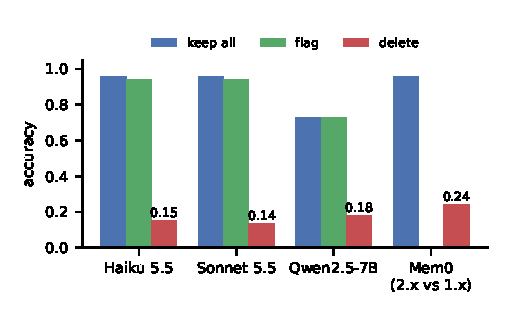
\includegraphics[width=\columnwidth]{../figures/history_by_policy.pdf}
\caption{Accuracy on the 66 history questions at 300 tokens. For Mem0, ``keep all'' is Mem0 2.x and
``delete'' is Mem0 1.x, which overwrites memories.}
\label{fig:history}
\end{figure}

\subsection{The same failure in a deployed system}
\label{sec:mem0}

Our policies share one pipeline, so we test whether the effect holds in a memory system built by
others. Mem0 \citep{chhikara2025mem0} changed its design between versions: Mem0 1.x runs an LLM update
step after each extraction that compares new facts with similar stored memories and decides to add,
update, delete or do nothing, while Mem0 2.x only adds memories. We run the open-source releases
(1.0.11 and 2.2.1) with the same extraction model (Haiku 5.5) and embedder, feed each history session
by session, retrieve with Mem0's own search, and pack, read and judge exactly as for our policies.
The open-source Mem0 does not store timestamps, so its memories are shown oldest first without dates.

On the original questions (Table~\ref{tab:ku}), the two versions tie on current questions (.88 each),
while Mem0 1.x answers .47 of the 15 history questions against .93 for Mem0 2.x (0--7, $p=.016$), the same
.47 as our own delete policy. On the 66 history questions the gap widens: Mem0 1.x answers .24 and Mem0
2.x .95 (48--1 for Mem0 2.x, $p<10^{-12}$; .23 vs .92 at 1000 tokens). Typical losses: asked ``How many engineers did
I lead when I started, and now?'', Mem0 1.x knows only the current 5; asked for a previous airline
status, it no longer has it. Mem0 1.x also scores below flagging overall (.81 vs .96, 0--12,
$p<.001$). Its update step occasionally refers to memory ids that do not exist (20 failed actions over
both runs), which Mem0 logs and skips; we report the system as released.

\subsection{Without dates, flagging is the best policy}
\label{sec:nodates}

Dates let the reader resolve conflicts itself, which is why flag adds nothing to keep in the dated
setting. Many memory systems do not keep dates on items (including the open-source Mem0 we tested),
so we also remove them (Table~\ref{tab:ku}, lower block). Keep then falls to .87 (Haiku), .90
(Sonnet) and .85 (Qwen), and flagging recovers much of the loss for the Claude readers (.95 and .94) and some for Qwen (.87). The direction is
the same for all three readers (Haiku 7--1, $p=.07$; Sonnet 4--1; Qwen 5--3), although no single
comparison is significant on 78 questions. Flag also beats delete without dates (Haiku 9--0,
$p=.004$). On history questions flag and keep remain tied (Table~\ref{tab:history}). The flag thus
does what deletion was meant to do, mark which value is current, without losing the earlier one.

\paragraph{Richer flags.} Naming the replacing item in the flag does not help further. Rich and plain
flags never differ significantly (with dates, Haiku 1--0, Sonnet 0--3, Qwen 0--1 on the original
questions; 2--1, 0--1, 5--5 on history questions). Without dates, the rich flag also improves on keep
in the same direction (Haiku .95 vs .87, 6--0, $p=.03$; Sonnet .92 vs .90, 3--1; Qwen .91 vs .85,
6--1). What matters is that the superseded item stays and is marked, not how the mark is worded.

\subsection{Other question types}

On LongMemEval's 266 temporal-reasoning and multi-session questions, which do not target updates,
the policies hardly differ at 300 tokens (keep .76, flag .76, delete .74), but at 1000 tokens deletion
again loses (.76 vs .80, 3--15, $p=.008$) while flag matches keep (.81). Flagging is therefore safe
beyond knowledge-update questions.

\section{Discussion}
\label{sec:discussion}

\paragraph{Is the result obvious?} It is unsurprising that deleted facts cannot be recalled. What
the results add is the price and the payoff: deletion buys nothing on current questions in any
setting we tested (at most one question net), costs about 80 points on questions about the past, and turns every link error into
a lost fact, while a deployed system made exactly this choice. Benchmarks that ask only for current
values hide the cost: our own earlier work, evaluated that way, concluded that deletion was the
solution, and recent work trains agents to overwrite \citep{patel2026supersede}. Our results do not
contradict that work, whose questions ask only for current values; they show what such training
optimises away.

\paragraph{Benchmarks rarely ask about the past.} LongMemEval has 13 answerable earlier-value
knowledge-update questions. LoCoMo has almost no superseded facts: mining both speakers of all ten
conversations with Sonnet 5.5 found 22 candidate changes, of which only 8 survived a check against
the cited dialogue turns (Appendix~\ref{app:locomo}). Evaluations of memory policies should include
questions about earlier values; our derived questions are a simple way to obtain them from any
benchmark with marked evidence for both values.

\paragraph{When might deletion still be right?} Deletion bounds memory growth and can serve privacy,
for example when a user asks to forget something. Those are reasons to delete on request or by
retention policy, not on supersession. When memory must shrink, flagged items can be summarised
(``previously X, until date'') rather than dropped. Superseded facts can also invalidate dependent
facts (a dropped country's deadline, \S\ref{sec:synthetic}), which a flag can express and deletion
cannot undo.

\section{Conclusion}

Deleting superseded facts looks ideal when only the present is queried. With predicted links and
questions about the past, it turns link errors and history questions into wrong answers, in our
pipeline and in Mem0. Flagging keeps what deletion was meant to provide, a clear signal of which value
is current, and it is the most accurate policy on the original update questions when memory has no dates. We recommend flagging
superseded facts rather than forgetting them, keeping dates on memory items, and evaluating memory on
questions about the past as well as the present.

\section*{Limitations}

Our main evaluation uses one benchmark, LongMemEval, whose 78 knowledge-update questions give wide
confidence intervals for differences between keep and flag; the deletion effects are large enough to
be clear. 53 of the 66 history questions are derived by an LLM from marked evidence; we checked each by hand
and release them with their evidence, but a single checker may miss errors. Every LongMemEval update has exactly two
values, so we cannot test chains of several updates, where a single flag may be less informative than
a dated history. Extraction, linking and judging use one model family (Claude); we mitigate this with
a second judge and an open-weight reader, but other extractors may link differently. We test two
wordings of the flag, not other presentations such as grouped version histories. The controlled benchmark
is templated and its updates are often explicit, so its detection results are optimistic. Mem0 is
tested in its open-source form, without timestamps.

\section*{Ethics Statement}

We use public research benchmarks whose conversations are synthetic or collected with consent; no
new personal data is collected. Retaining superseded facts keeps more information about users;
deployed systems should still delete on user request and follow retention policies.

\bibliography{custom}

\appendix

\section{Prompts}
\label{app:prompts}

All prompts are released with the code; we summarise them here.
\textbf{Extraction.} Self-contained, specific items with exact values about the user and people close
to them, including details mentioned in passing; skip generic requests and pasted content; a type and
an optional due date. \textbf{Link detection.} A new item \emph{replaces} an earlier item only when
the earlier one is no longer true (a changed number, a new personal best, a move, a reversed
decision); two different events, or a fact that adds detail, are not replacements. Output:
\texttt{\{"replacements": [\{"new\_id", "replaced\_ids"\}]\}}. \textbf{Reader.} Answer from memory;
when values conflict, the most recently stated one is current; say you don't know if the memory
does not contain the answer; one or two sentences. \textbf{Judge.} Current questions: correct if the
response contains the gold answer; mentioning earlier information is acceptable if the updated value
is given as current. History questions: correct if the response gives the earlier value. Abstention
questions: correct only if the response says the information is unknown. \textbf{History question
generation.} Given the dated evidence turns and the original question and answer, write a question
asking for the value before the change, which refers to the change so it has one clear answer and
does not contain the earlier value; mark it unusable if the earlier value is not stated explicitly.

\section{LoCoMo}
\label{app:locomo}

For each of the 20 speakers in LoCoMo's ten conversations, Sonnet 5.5 read that speaker's dated
session observations and listed facts whose value was stated and later replaced, with the dialogue
turns that state each value. A second call checked each candidate against the two cited turns. Of 22
candidates, 8 were confirmed; most rejected ones cited turns that did not state the claimed value
explicitly. The 16 resulting questions (current and earlier value) are too few to compare policies:
keep, flag and delete are within two answers of each other.

\section{Implementation Details}

Models: Claude Haiku 5.5 (\texttt{claude-haiku-5-5}) and Claude Sonnet 5.5
(\texttt{claude-sonnet-5-5}) with effort ``medium'' (judge ``low'') and structured JSON outputs;
Qwen2.5-7B-Instruct via Ollama, temperature 0. Token budgets use the \texttt{cl100k\_base}
tokenizer. User turns are truncated to 3,000 characters and sessions to 12,000 characters before
extraction. The extraction prompt was revised once, after a three-question pilot showed that it
skipped facts about the user's friends. Mem0 uses the same extraction model, all-MiniLM-L6-v2
embeddings and a local Qdrant store; we retrieve its top 50 memories and pack them into the same
budgets. All model responses are cached, so every table can be regenerated without new calls.

\end{document}
